\documentclass[aspectratio=169]{beamer}

% =============================
% PACOTES ESSENCIAIS
% =============================
\usepackage[utf8]{inputenc}
\usepackage[T1]{fontenc}
\usepackage{graphicx}
\usepackage{booktabs}
\usepackage{amsmath, amsfonts, amssymb}
\usepackage{tikz}
\usepackage{pgfplots}
\usepackage{lmodern}
\usepackage{ragged2e}
\usepackage{microtype}

\pgfplotsset{compat=1.18}

% =============================
% PALETA DE CORES (AURUM)
% =============================
\definecolor{AurumDark}{RGB}{22,22,22}
\definecolor{AurumGold}{RGB}{180,140,60}
\definecolor{AurumGray}{RGB}{120,120,120}
\definecolor{AurumLight}{RGB}{245,245,245}

% =============================
% FONTES
% =============================
\usefonttheme{professionalfonts}
\setbeamerfont{title}{series=\bfseries,size=\Large}
\setbeamerfont{frametitle}{series=\bfseries,size=\large}
\setbeamerfont{normal text}{size=\normalsize}

% =============================
% LAYOUT GLOBAL
% =============================
\setbeamercolor{background canvas}{bg=AurumLight}
\setbeamercolor{normal text}{fg=AurumDark}
\setbeamercolor{frametitle}{fg=AurumDark}
\setbeamercolor{title}{fg=AurumDark}

\setbeamercolor{block title}{fg=AurumLight,bg=AurumDark}
\setbeamercolor{block body}{fg=AurumDark,bg=white}

\setbeamercolor{alertblock title}{fg=white,bg=AurumGold}
\setbeamercolor{alertblock body}{fg=AurumDark,bg=white}

% =============================
% REMOVER ÍCONES PADRÃO
% =============================
\setbeamertemplate{navigation symbols}{}

% =============================
% RODAPÉ MODERNO
% =============================
\setbeamertemplate{footline}{
\leavevmode%
\hbox{
\begin{beamercolorbox}[wd=.8\paperwidth,ht=2.5ex,dp=1ex,left]{author in head/foot}
\hspace{1em}\textcolor{AurumGray}{\insertshortauthor}
\end{beamercolorbox}
\begin{beamercolorbox}[wd=.2\paperwidth,ht=2.5ex,dp=1ex,right]{date in head/foot}
\textcolor{AurumGray}{\insertframenumber{}\ /\ \inserttotalframenumber}\hspace{1em}
\end{beamercolorbox}}
}

% =============================
% TÍTULO DE SLIDE COM LINHA
% =============================
\setbeamertemplate{frametitle}{
\vspace{0.5em}

\begin{tikzpicture}
\node[anchor=west] at (0,0) {\insertframetitle};
\draw[AurumGold, thick] (0,-0.3) -- (\paperwidth,-0.3);
\end{tikzpicture}
\vspace{1em}
}

% =============================
% INFORMAÇÕES
% =============================
\title{Apresentação de Teste}
\subtitle{Design AURUM Minimal Beamer}
\author{Autor Exemplo}
\institute{Instituição Exemplo}
\date{\today}

% =============================
% DOCUMENTO
% =============================
\begin{document}

% -----------------------------
% CAPA
% -----------------------------
\begin{frame}[plain]
\vfill
\begin{center}
{\Huge\bfseries \inserttitle}

\vspace{0.5em}

{\large\textcolor{AurumGray}{\insertsubtitle}}

\vspace{2em}

{\insertauthor}

\vspace{0.5em}

{\small\textcolor{AurumGray}{\insertinstitute}}

\vspace{2em}

\textcolor{AurumGold}{\rule{0.6\textwidth}{1pt}}
\end{center}
\vfill
\end{frame}

% -----------------------------
% SUMÁRIO
% -----------------------------
\begin{frame}{Estrutura}
\tableofcontents
\end{frame}

% -----------------------------
\section{Introdução}

\begin{frame}{Introdução}
\justifying
Esta apresentação demonstra um design inovador em \LaTeX\ utilizando o Beamer,
com foco em clareza visual, elegância e hierarquia de informação.
\end{frame}

% -----------------------------
\section{Texto}

\begin{frame}{Texto e Parágrafo}
O \LaTeX\ é amplamente utilizado na produção científica por oferecer controle
preciso de layout, tipografia profissional e consistência visual.
\end{frame}

% -----------------------------
\begin{frame}{Lista}
\begin{itemize}
\item Organização visual
\item Elegância tipográfica
\item Estrutura clara
\item Uso acadêmico avançado
\end{itemize}
\end{frame}

% -----------------------------
\section{Matemática}

\begin{frame}{Fórmula}
\[
E = mc^2
\]
\end{frame}

\begin{frame}{Cálculo}
\[
\int_a^b f(x)\,dx = F(b)-F(a)
\]
\end{frame}

% -----------------------------
\section{Blocos}

\begin{frame}{Definição}
\begin{block}{Função}
Uma função associa cada elemento de um conjunto a exatamente um elemento de outro.
\end{block}
\end{frame}

\begin{frame}{Alerta}
\begin{alertblock}{Atenção}
Design bom é invisível — ele serve ao conteúdo.
\end{alertblock}
\end{frame}

% -----------------------------
\section{Tabelas}

\begin{frame}{Tabela}
\centering
\begin{tabular}{l c c}
\toprule
Item & A & B \\
\midrule
X & 10 & 20 \\
Y & 15 & 25 \\
Z & 30 & 40 \\
\bottomrule
\end{tabular}
\end{frame}

% -----------------------------
\section{Gráficos}

\begin{frame}{Gráfico}
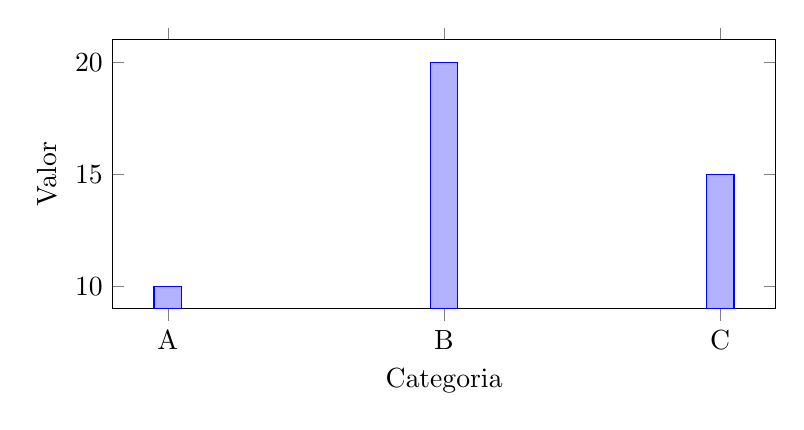
\begin{tikzpicture}
\begin{axis}[
ybar,
height=5cm,
width=10cm,
ylabel={Valor},
xlabel={Categoria},
symbolic x coords={A,B,C},
xtick=data
]
\addplot coordinates {(A,10) (B,20) (C,15)};
\end{axis}
\end{tikzpicture}
\end{frame}

% -----------------------------
\section{Conclusão}

\begin{frame}{Conclusão}
O design \textbf{AURUM Minimal Beamer} prova que apresentações em \LaTeX\ podem ser
sofisticadas, modernas e altamente profissionais.
\end{frame}

% -----------------------------
\begin{frame}[plain]
\vfill
\begin{center}
{\Huge Obrigado!}

\vspace{1em}

{\Large Perguntas?}
\end{center}
\vfill
\end{frame}

\end{document}
